% ============================================================
%  sec-3-huawei-overview.tex  —  1.3 Huawei Group Overview
% ============================================================

\section{Huawei Group Overview}
\label{sec:huawei-overview}

% ── 1.3.1 ────────────────────────────────────────────────────
\subsection{Introduction to Huawei}
\label{subsec:huawei-intro}

Huawei Investment \& Holding Co., Ltd.\ is a Chinese multinational corporation
specialising in the research, development, manufacturing, and marketing of
\acrfull{ict} infrastructure and smart devices. Founded in 1987 by Ren Zhengfei
in Shenzhen and wholly owned by its 169,054 employee-shareholders, Huawei
operates across more than 170 countries with approximately 213,000 employees
and serves over 3 billion people globally.

The company's overarching mission is to \textit{``bring digital to every person,
home, and organisation for a fully connected, intelligent world''}, emphasising
AI as a universal technology comparable to water and electricity for all
industries.

\begin{figure}[H]
    \centering

    \begin{subfigure}{0.4\textwidth}
        \centering
        \includegraphics[width=\linewidth]{images/logos/Huawei-logo.jpg}
        \caption{Company Logo}
    \end{subfigure}
    \hfill
    \begin{subfigure}{0.5\textwidth}
        \centering
        \includegraphics[width=\linewidth]{images/logos/headquarter.jpg}
        \caption{Company Headquarters}
    \end{subfigure}

    \caption{Company Identity and Headquarters}
    \label{fig:company_overview}
\end{figure}

\subsubsection{Strategic Positioning}
\label{subsubsec:strategic-positioning}

Huawei has positioned itself at the convergence of \acrshort{ict}
infrastructure, AI computing, and cloud services under an ``All Intelligence
Strategy''. Its core strategic priorities are summarised in
\tabref{huawei-strategic-priorities}.

\begin{table}[htbp]
  \centering
  \caption{Huawei's key strategic priorities (2025)}
  \label{tab:huawei-strategic-priorities}
  \begin{tabularx}{0.92\textwidth}{>{\bfseries}lX}
    \toprule
    \tableheader{Strategic Priority & Description} \\
    \midrule
    AI-First Approach     & Full investment in Ascend \acrshort{npu}s,
                            Kunpeng processors, and Pangu AI models \\
    \rowcolor{TableRowOdd}
    5G/5G-A Leadership    & Supporting 230+ carriers worldwide; 5G-A users
                            exceeded 60 million in 2025 \\
    Cloud Computing       & Huawei Cloud deployed in 29 regions globally,
                            serving 500+ scenarios across 30+ industries \\
    \rowcolor{TableRowOdd}
    Computing Ecosystem   & Kunpeng: 3.8 M developers; Ascend: 4 M developers
                            (2025) \\
    Open Collaboration    & 9,800+ partners; 26,000+ industry solutions \\
    \bottomrule
  \end{tabularx}
\end{table}

% ── 1.3.2 ────────────────────────────────────────────────────
\subsection{Historical Background and Evolution}
\label{subsec:huawei-history}

Huawei's 38-year evolution from a small telecommunications switch reseller to
a global technology powerhouse is characterised by aggressive R\&D investment,
strategic international expansion, and remarkable resilience under geopolitical
pressure. \tabref{huawei-timeline} presents the key milestones of this
trajectory.

\begin{table}[htbp]
  \centering
  \caption{Selected milestones in Huawei's corporate history}
  \label{tab:huawei-timeline}
  \begin{tabularx}{\textwidth}{>{\bfseries}lX}
    \toprule
    \tableheader{Year & Milestone} \\
    \midrule
    1987 & Founded in Shenzhen with RMB 21,000 capital; initially reselling PBX switches \\
    \rowcolor{TableRowOdd}
    1993 & Launched C\&C08 program-controlled telephone switch — most powerful in China at the time \\
    1997 & First international contract (Hutchison Whampoa, Hong Kong); entered wireless GSM \\
    \rowcolor{TableRowOdd}
    2005 & International revenue exceeded domestic sales for the first time \\
    2010 & First inclusion in Fortune Global 500 (revenue: \$21.8B) \\
    \rowcolor{TableRowOdd}
    2012 & Surpassed Ericsson to become world's largest telecommunications equipment manufacturer \\
    2019 & US Entity List designation; launched Ascend 910 (256 TFLOPS FP16 at 310W)
           and HarmonyOS \\
    \rowcolor{TableRowOdd}
    2024 & Revenue CN¥862.1B (\$118.1B), 22\% year-on-year growth despite sanctions \\
    2025 & Ascend 910C mass-produced (SMIC N+2); Ascend ecosystem: 4M developers;
           ranked \#83 in Fortune Global 500 \\
    \bottomrule
  \end{tabularx}
\end{table}


\subsubsection{AI Computing Roadmap}
\label{subsubsec:ai-roadmap}

Huawei's AI computing strategy, detailed in \tabref{ascend-roadmap}, follows a
one-year release cadence with the goal of doubling compute performance per
generation.

\begin{table}[htbp]
  \centering
  \caption{Huawei Ascend NPU product roadmap}
  \label{tab:ascend-roadmap}
  \begin{tabularx}{\textwidth}{lllX}
    \toprule
    \tableheader{Model & Year & Performance & Key Significance} \\
    \midrule
    Ascend 310  & 2018      & Inference-focused  & First AI chip in Ascend series \\
    \rowcolor{TableRowOdd}
    Ascend 910  & Aug.~2019 & 256 TFLOPS (FP16) & World's most powerful AI processor at launch \\
    Ascend 910C & Q1 2025   & 800 TFLOPS (FP16) & SMIC N+2 process; powers DeepSeek AI models \\
    \rowcolor{TableRowOdd}
    Ascend 950  & 2026      & TBD               & Two-variant next-generation chip \\
    Ascend 960  & 2027      & TBD               & Continued AI chip roadmap \\
    \rowcolor{TableRowOdd}
    Ascend 970  & 2028      & TBD               & Targeting 4 zettaFLOPS (FP4) at system level \\
    \bottomrule
  \end{tabularx}
\end{table}


% ── 1.3.4 ────────────────────────────────────────────────────
\subsection{Organisational Structure and Business Divisions}
\label{subsec:huawei-structure}

Huawei operates under a unique employee-ownership governance model combining
strategic board oversight with rotating executive leadership. The Rotating
Chair system — in which the CEO role rotates on six-month terms among senior
executives — is designed to prevent concentration of authority and enhance
organisational resilience under geopolitical pressure.

\begin{figure}[H]
    \centering
    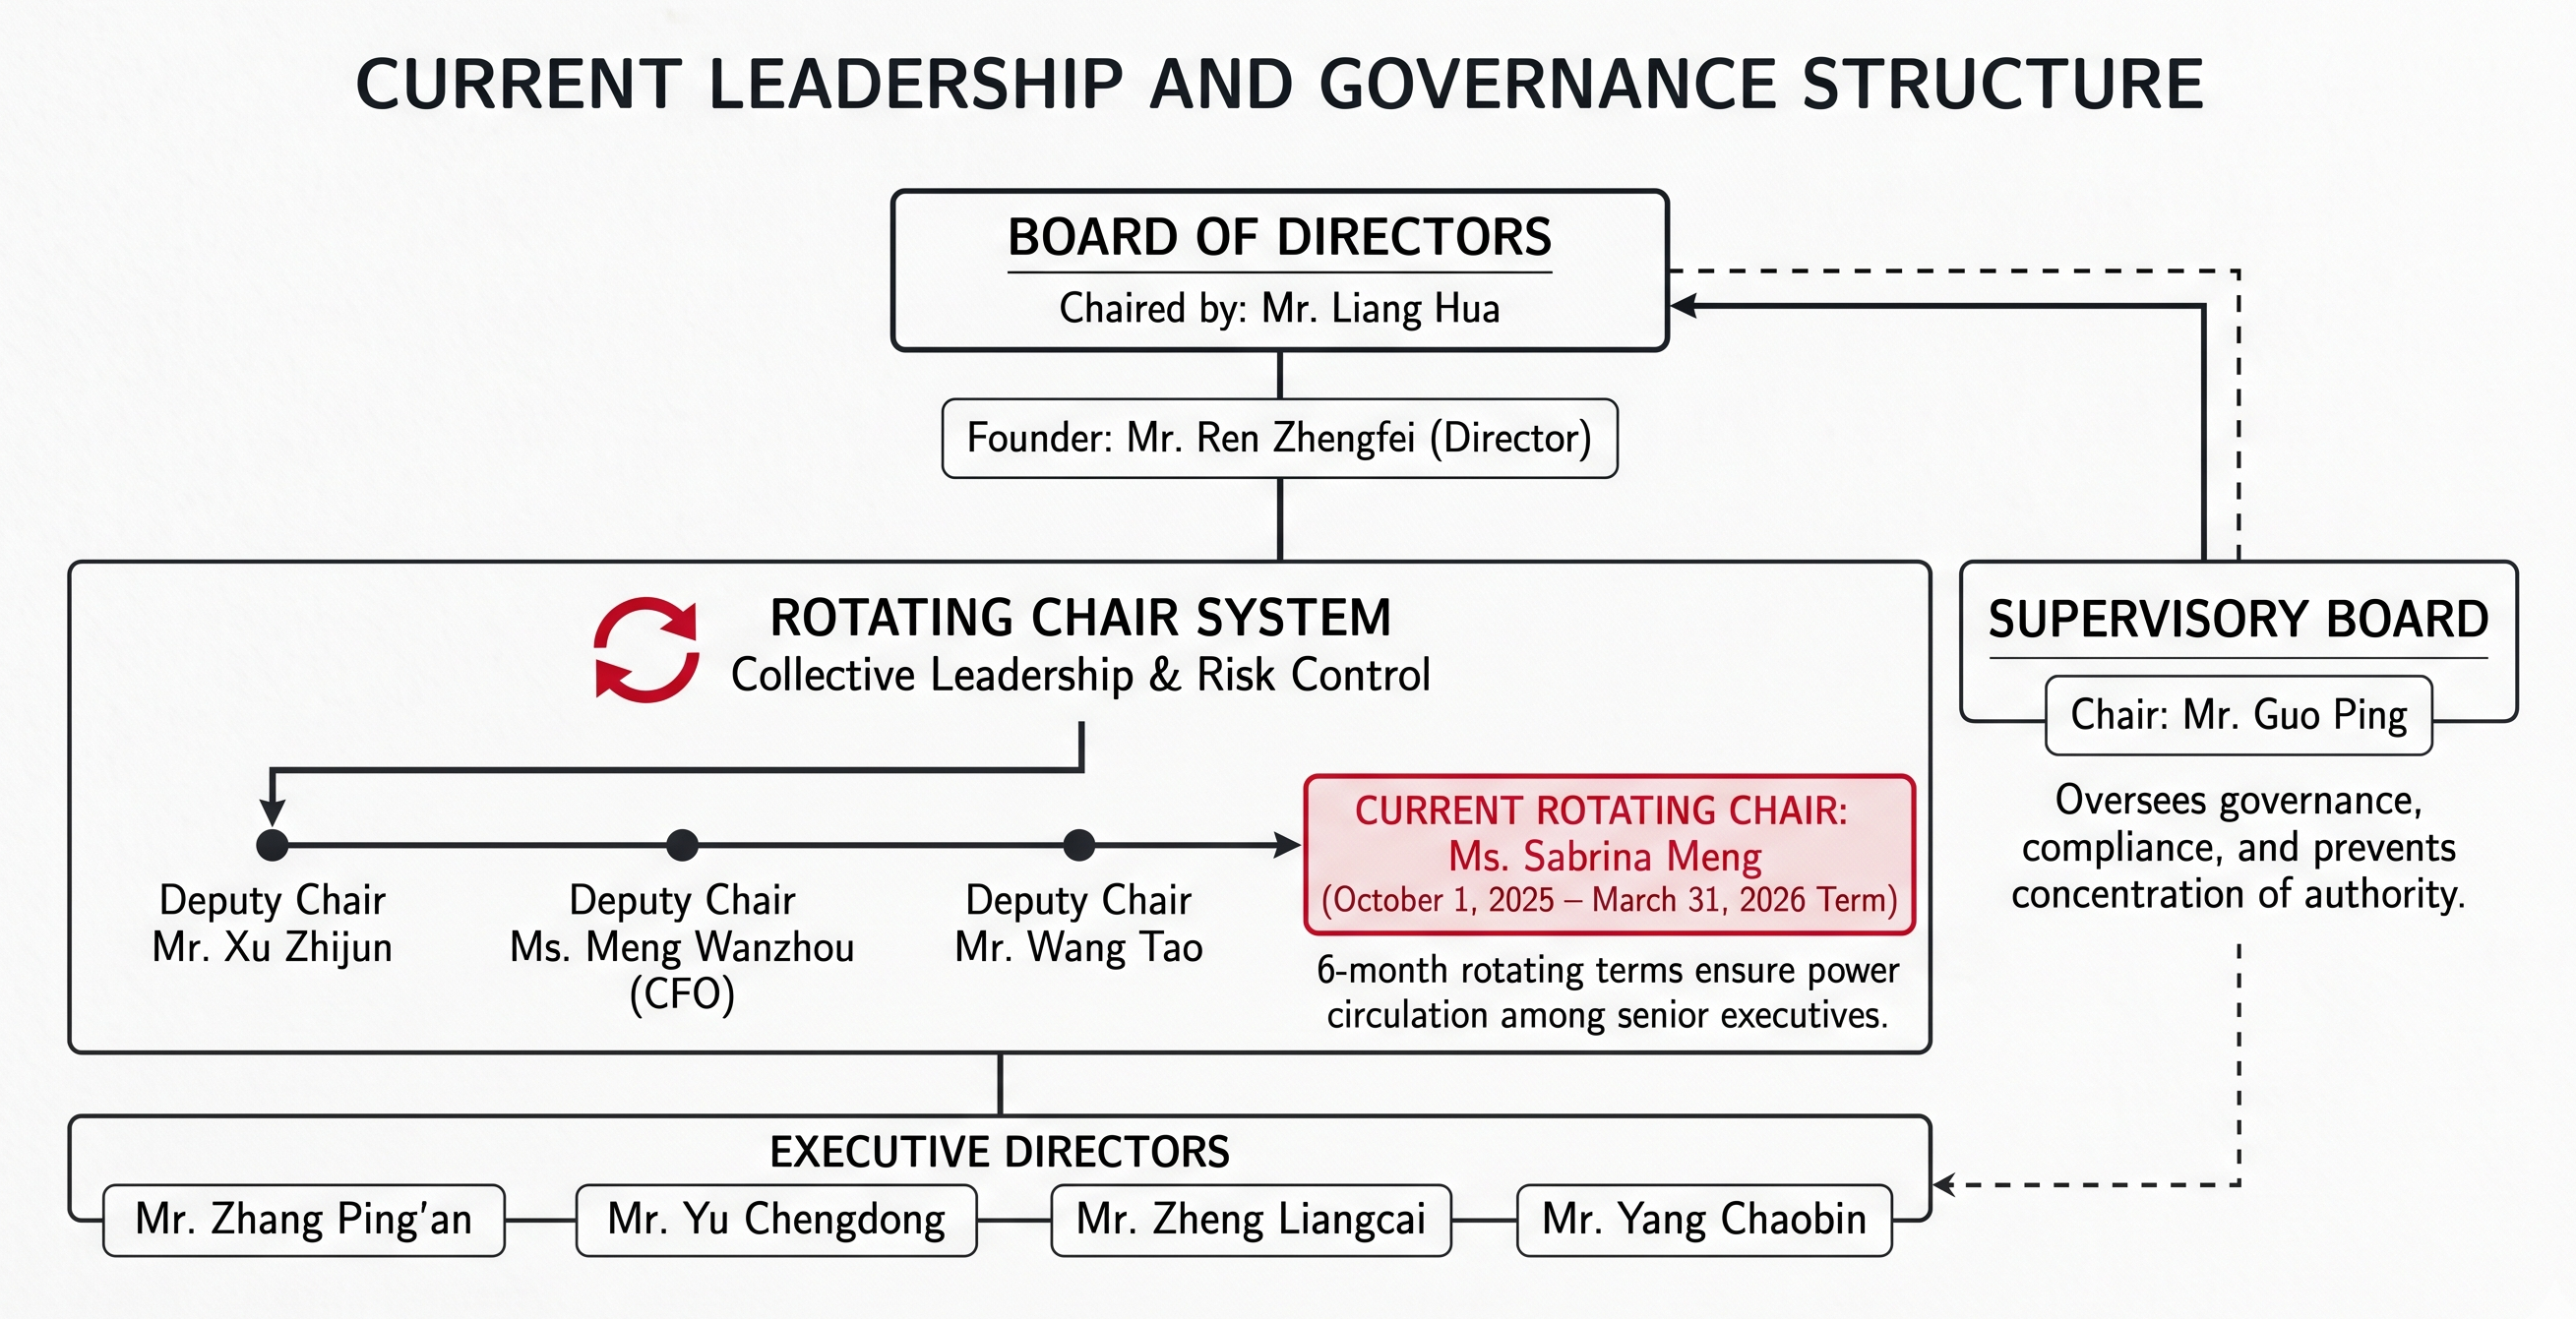
\includegraphics[width=0.8\textwidth]{images/figures/deputy-chairs.png}
    \caption{Rotating Chair System Overview }
    \label{fig:Rotating Chair System Overview }
\end{figure} 


Huawei's operations are organised into four primary Business Groups plus
specialised divisions, as summarised in \tabref{business-groups}.

\begin{table}[htbp]
  \centering
  \caption{Huawei business divisions and key products}
  \label{tab:business-groups}
  \begin{tabularx}{\textwidth}{lX}
    \toprule
    \tableheader{Division & Focus \& Key Products} \\
    \midrule
    Carrier Business Group (\acrshort{cbg})
      & Telecommunications infrastructure: 5G/5G-A base stations, optical
        networks, core networks. Serves 230+ operators worldwide. \\
    \rowcolor{TableRowOdd}
    Enterprise Business Group (\acrshort{ebg})
      & Enterprise \acrshort{ict}: data centres (FusionCube, OceanStor), enterprise
        networking, private 5G, industry cloud solutions. \\
    Consumer Business Group
      & Smart devices: Huawei smartphones (Pura, Mate series), HarmonyOS,
        wearables, tablets. 900M+ HarmonyOS devices (June 2024). \\
    \rowcolor{TableRowOdd}
    Huawei Cloud
      & Public cloud, AI services (Ascend-based instances), industry cloud.
        29 regions globally, 500+ industry scenarios. \\
    AI \& Computing (HiSilicon)
      & Ascend \acrshort{npu}s, Kunpeng processors, MindSpore, \acrshort{cann}.
        Core of Huawei's post-sanctions technological independence strategy. \\
    \rowcolor{TableRowOdd}
    Digital Power
      & Solar inverters, energy storage, EV charging, data centre power systems. \\
    \bottomrule
  \end{tabularx}
\end{table}

% ── 1.3.5 ────────────────────────────────────────────────────
\subsection{Technologies, Products, and Innovation}
\label{subsec:huawei-tech}

Huawei's portfolio spans telecommunications infrastructure, AI computing,
cloud services, consumer devices, and digital power solutions. Key product
families directly relevant to this project are described below.


The Ascend \acrshort{npu} series forms the centrepiece of Huawei's AI computing
strategy. CANN (Compute Architecture for Neural Networks) serves as Huawei's
software abstraction layer analogous to NVIDIA's \acrshort{cuda}, while
MindSpore is an open-source AI training and inference framework supporting
Ascend-native execution. With 4 million developers in the Ascend ecosystem
(2025), Huawei has established a viable alternative to the NVIDIA stack for
Chinese AI infrastructure.

% ── 1.3.6 ────────────────────────────────────────────────────
\subsection{Research \& Development}
\label{subsec:huawei-rd}

Huawei's R\&D commitment is among the most intensive globally. In 2025, the
company invested CNY 192.3 billion (US\$27.5B), representing 21.8\% of annual
revenue — one of the highest R\&D-to-revenue ratios in the global technology
industry. \tabref{rd-investment} summarises recent investment levels.

\begin{table}[htbp]
  \centering
  \caption{Huawei annual R\&D investment (selected years)}
  \label{tab:rd-investment}
  \begin{tabularx}{0.88\textwidth}{lllr}
    \toprule
    \tableheader{Year & R\&D Investment & \% of Revenue & R\&D Employees} \\
    \midrule
    2022 & CNY 161.5B  & 25.1\% & 114,000 \\
    \rowcolor{TableRowOdd}
    2024 & CNY 170.0B  & 21.0\% & 117,150 \\
    2025 & CNY 192.3B  & 21.8\% & 114,000 \\
    \bottomrule
  \end{tabularx}
\end{table}

Huawei has ranked \#1 globally in PCT patent applications for nine consecutive
years (2014–2024), with 165,000+ active granted patents and US\$630 million in
patent licensing revenue in 2024.

% ── 1.3.7 ────────────────────────────────────────────────────
\subsection{Huawei Morocco and Internship Context}
\label{subsec:huawei-morocco}

Huawei has maintained a presence in Morocco since 2007, establishing the
country as the strategic hub for its Northern Africa operations — covering
North, West, and Central Africa. Under the ``In Morocco, For Morocco''
philosophy, Huawei Morocco (Huawei Technologies Morocco S.a.r.l.) serves
as the regional headquarters and actively contributes to Morocco's digital
transformation under the Digital Morocco 2030 programme.


Huawei has partnered with Maroc Telecom, Orange Morocco, and Inwi for 4G/5G
infrastructure deployment — Morocco officially entered the 5G era on
November~7, 2025. The company also supports 54 partner universities through
the Huawei ICT Academy programme, targeting 1,100+ certified students by
2025–2026 across AI, cloud, 5G, and cybersecurity disciplines.

At the 2024 Digital Africa Summit in Marrakech, Huawei committed US\$500M over
five years to expand cloud coverage across Africa, reflecting Morocco's central
role in its continental strategy.
